% $Id: template.tex 11 2007-04-03 22:25:53Z jpeltier $

\documentclass{vgtc}                          % final (conference style)
%\documentclass[review]{vgtc}                 % review
%\documentclass[widereview]{vgtc}          % wide-spaced review
%\documentclass[preprint]{vgtc}               % preprint
%\documentclass[electronic]{vgtc}             % electronic version

%% Uncomment one of the lines above depending on where your paper is
%% in the conference process. ``review'' and ``widereview'' are for review
%% submission, ``preprint'' is for pre-publication, and the final version
%% doesn't use a specific qualifier. Further, ``electronic'' includes
%% hyperreferences for more convenient online viewing.

%% Please use one of the ``review'' options in combination with the
%% assigned online id (see below) ONLY if your paper uses a double blind
%% review process. Some conferences, like IEEE Vis and InfoVis, have NOT
%% in the past.

%% Figures should be in CMYK or Grey scale format, otherwise, colour 
%% shifting may occur during the printing process.

%% These three lines bring in essential packages: ``mathptmx'' for Type 1 
%% typefaces, ``graphicx'' for inclusion of EPS figures. and ``times''
%% for proper handling of the times font family.

\usepackage{mathptmx}
\usepackage{graphicx}
\usepackage{times}
\usepackage{cite} 
\usepackage{subcaption}

%% We encourage the use of mathptmx for consistent usage of times font
%% throughout the proceedings. However, if you encounter conflicts
%% with other math-related packages, you may want to disable it.

%% If you are submitting a paper to a conference for review with a double
%% blind reviewing process, please replace the value ``0'' below with your
%% OnlineID. Otherwise, you may safely leave it at ``0''.
\onlineid{0}

%% declare the category of your paper, only shown in review mode
\vgtccategory{Research}

%% allow for this line if you want the electronic option to work properly
\vgtcinsertpkg

%% In preprint mode you may define your own headline.
%\preprinttext{To appear in an IEEE VGTC sponsored conference.}

%% Paper title.

\title{An approach for Ray Tracing on Exascale Computers}

%% This is how authors are specified in the conference style

%% Author and Affiliation (single author).
%%\author{Roy G. Biv\thanks{e-mail: roy.g.biv@aol.com}}
%%\affiliation{\scriptsize Allied Widgets Research}

%% Author and Affiliation (multiple authors with single affiliations).
\author{
  Ellen A. Porter
  \thanks{e-mail: \texttt{ellen.porter@wsu.edu}} %
  \and
  Robert R. Lewis
  \thanks{e-mail: \texttt{bobl@tricity.wsu.edu}}}

\affiliation{
  \scriptsize Washington State University, Tri-Cities \\
  Program in Engineering and Computer Science}

%% Author and Affiliation (multiple authors with multiple affiliations)
%%\author{Roy G. Biv\thanks{e-mail: roy.g.biv@aol.com}\\ %
%%        \scriptsize Starbucks Research %
%%\and Ed Grimley\thanks{e-mail:ed.grimley@aol.com}\\ %
%%     \scriptsize Grimley Widgets, Inc. %
%%\and Martha Stewart\thanks{e-mail:martha.stewart@marthastewart.com}\\ %
%%     \parbox{1.4in}{\scriptsize \centering Martha Stewart Enterprises \\ Microsoft Research}}

%% A teaser figure can be included as follows, but is not recommended since
%% the space is now taken up by a full width abstract.
%\teaser{
%  \includegraphics[width=1.5in]{sample.eps}
%  \caption{Lookit! Lookit!}
%}

%% Abstract section.
\abstract{
Exascale computers, defined as being capable of performing at least one exaflop ($10^{18}$ floating point operations per second) are anticipated to emerge in the next several years.  Reaching this scale of computation will require significant hardware and software changes for high-performance computing (HPC).  Applications will need to adapt as the architecture of supercomputers change.  In this paper we explore those changes and the impact they will have on programming models and application design.  We then  look at one specific model, the Concurrent Collections Programming Model (CnC) and explore how we can use CnC and Intel's Embree Ray Tracing Engine to build a scalable ray tracing system ready for exascale.

} % end of abstract

%% ACM Computing Classification System (CCS). 
%% See <http://www.acm.org/class/1998/> for details.
%% The ``\CCScat'' command takes four arguments.

\CCScatlist{ 
\CCScat{}{Computing methodologies}{Ray tracing}{}
\CCScat{}{Computing methodologies}{Parallel programming languages}{}
\CCScat{}{Hardware}{Emerging architectures}{}
}

%% Copyright space is enabled by default as required by guidelines.
%% It is disabled by the 'review' option or via the following command:
% \nocopyrightspace

%%%%%%%%%%%%%%%%%%%%%%%%%%%%%%%%%%%%%%%%%%%%%%%%%%%%%%%%%%%%%%%%
%%%%%%%%%%%%%%%%%%%%%% START OF THE PAPER %%%%%%%%%%%%%%%%%%%%%%
%%%%%%%%%%%%%%%%%%%%%%%%%%%%%%%%%%%%%%%%%%%%%%%%%%%%%%%%%%%%%%%%%

\begin{document}

%% The ``\maketitle'' command must be the first command after the
%% ``\begin{document}'' command. It prepares and prints the title block.

%% the only exception to this rule is the \firstsection command

\firstsection{Introduction}

\maketitle

%% \section{Introduction} 

Achieving the performance expected from an exascale computer will require modifications to current hardware architecture which will in turn affect programming models and runtime design.  Until recent years, performance has increased in line with Moore's law, the number of transistors within an integrated circuit doubled approximately every two years.  As we reached a limit on the number of transistors a single chip could contain, hardware architects had to look for other ways to keep up with performance advancement expectations.  In order to take advantage of these hardware advances applications often required redesign. 

In addition to the changing algorithms, the data produced as output from high-performance computing (HPC) applications tends to scale in size with compute power.  This has produced a need for visualization algorithms that can take advantage of distributed systems as well as an opportunity to design algorithms that can be integrated into HPC applications to produce results during execution.  This paper proposes one such design for ray tracing, a commonly used rendering technique, using the Intel Concurrent Collections (CnC) programming model.   


\section{Reaching Exascale}

For the past two decades high performance computing (HPC) progression has been driven by Moore's law which states microprocessor performance and memory chip density increase exponentially over time.  Until 2004, performance of single-core microprocessors increased as predicted as a result of smaller and faster transistors being developed.  In 2004 this advancement trend shifted as we reached an inflection point caused by a chip’s power dissipation ~\cite{kogge2013exascale}.  Unable to sufficiently and inexpensively cool a chip, chip designers looked for other ways to increase performance.  This came in the form of multi-core processors which are now the building blocks of many HPC systems.

The introduction of multi-core processors on a single node of a cluster caused a shift in parallel application design.  Message Passing Interface (MPI) programs could not exploit the parallelism on a single node without a rewrite of the underlying algorithms.  This resulted in the emergence of hybrid systems that mix MPI and OpenMP, each node executing an OpenMP program being controled by an MPI process.  The OpenMP program then uses a fixed number of threads to execute a single work-sharing construct such as a parallel loop ~\cite{gropp2013programming}.

As we look towards the next generation of HPC systems a shift in application design will once again be necessary to reach exascale performance.  On-chip parallelism along with reduced data movement will be critical for an applications success.  Unfortunately, conventional language semantics will not be sufficient to exploit the architecture advances being developed such as inter-core message queues.  Therefore, new high-performance parallel programming models and smarter runtimes are being developed.  The majority of these models are data-centric rather than compute-centric, which allows the runtime scheduler to prioritize scheduling computation on nodes or cores where the required data already resides rather than the next available processor ~\cite{kogge2013exascale}.  This kind of model will reduce communication which is the predicted bottle neck for exascale systems.

\section{CnC Programming Model}

The Concurrent Collections Programming Model (CnC) is a data-centric programming model, the deterministic semantics of which allow a task-based runtime to programmatically exploit parallelism.  In this model, algorithms are designed based on their data dependencies and control dependencies ~\cite{budimlicconcurrent}.  The specifics regarding the execution of the algorithm is then abstracted out of the implementation.  This allows the runtime to optimally decide when and where to schedule computation.  Hints can also be provided to the runtime through a separate file called a tuning specification.  

The CnC model is built on three key constructs; step collections, data collections, and control collections ~\cite{budimlicconcurrent}.  A step collection defines computation, an instance of which consumes and produces data.  The consumed and produced data, or data items, belong to data collections.  Data items within a data collection are indexed using item tags.  Finally the control collection describes the prescription, or creation, of step instances.  The relationship between these three collections is defined statically in an input file called a CnC graph.

Developing a CnC application begins with designing the CnC graph file.  An algorithm is broken down into computation steps, instances of which correspond to different input arguments.  These steps along with the data collections become nodes in a graph.  Each step can optionally consume data, produce data, and prescribe additional computation.  These relationships, producer, consumer, and control, define the edges in the graph and will dynamically be satisfied as the program executes.

\begin{figure*}[!htb]
  \centering
  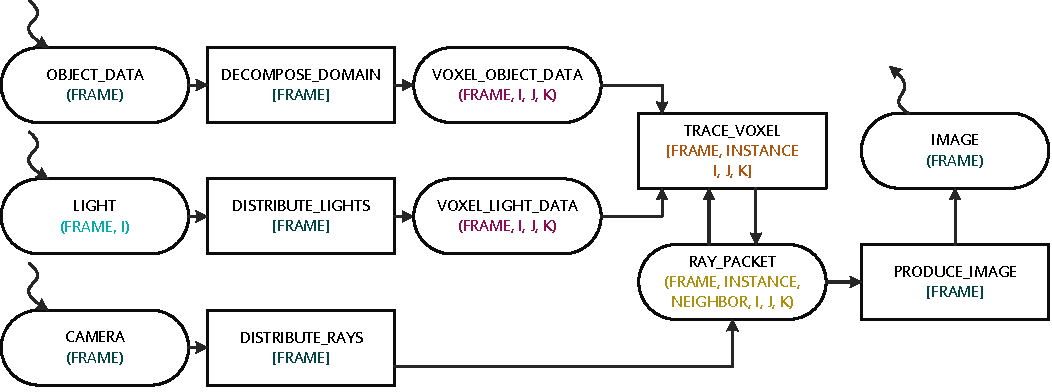
\includegraphics[width=\textwidth]{drawings/CnC.pdf}
  \caption{CnC graph}
  \label{fig:cnc}
\end{figure*}

The next and final required step in producing a CnC application is to implement the step logic.  The flow within a single CnC step is as follows: consume, compute and produce.  This ordering is required as there is no guarantee the data a step needs will be ready when the step beings executing.  Internally, CnC will attempt to retrieve the data, if it is not ready, the step will halt execution and try again later.  To improve performance, hints can be provided through the tuning specification to ensure steps are only prescribed and scheduled for execution when their required input data is ready.

\section{Current Ray Tracing Algorithms}

Traditional ray tracing algorithms are embarrassingly parallel as no ray depends on any other ray.  The data needed by each individual ray however varies widely as its path is traced.   Acceleration structures, such as k-d trees have been developed to increase ray tracing performance.  As the data scales up however, it is no longer possible to store an entire data set in an acceleration structure in shared memory.  One solution is to implement data decomposition.  Each node on a distributed system is then responsible for a subset of the domain.   Primary rays and secondary rays are then communicated across nodes as the algorithm executes.  These types of models typically rely on expensive preprocessing steps that help to balance both the data distribution and rendering work evenly across nodes ~\cite{navratil2014dynamic}. 

\section{CnC Ray Tracing Implementation}
Implementing ray tracing using CnC allows the algorithm to run on a distributed system and reduces the need for expensive preprocessing seen with many current systems.  This is due to the dynamic nature of CnC execution and is similar to the algorithm proposed by Navratil et al. ~\cite{navratil2014dynamic}.  The CnC implementation beings by splitting data into voxels, this data is then distributed dynamically at runtime.  The ray tracing portion of the algorithm is iterative.  Primary rays are sent into the system from the camera and then passed between neighboring voxels until all rays are fully traced.

Figure \ref{fig:cnc} shows the proposed CnC graph for distributed ray tracing.  Data collections, step collections and the dependencies between them are represented in the graph.  The tags corresponding to each collection are shown within the graph node.  The control collection for the proposed model is static for all steps except trace voxel and defined in an initialization step.  The graph begins execution when the object data, light data, and camera data are provided, and terminates when it produces an image.

\subsection{Tag Collections}

The tag collections are different for most data and step collections but share common elements.  FRAME refers to one specific frame in the case of an animation.  INSTANCE refers to the current iteration. I, J, K are iterators over spatial data, or in the case of LIGHT, the light index.

\subsection{Data Collections}

OBJECT\_DATA contains input data for the scene from the environment.  It is in the form of .obj.  DECOMPOSE\_DOMAIN splits this data into voxels and produces VOXEL\_OBJECT\_DATA.  Triangles that span multiple voxels are duplicated.  The LIGHT data collection contains data pertaining to any light sources.  VOXEL\_LIGHT\_DATA contains the same information as LIGHT plus a traced light mesh for each wall of a voxel.  CAMERA contains the location and direction of the camera.  RAY\_PACKET contains all the rays that intersect a voxel wall for a given wall and iteration.  IMAGE contains the final image data.


\subsection{Step Collections}

\subsubsection{Decompose Domain}

DECOMPOSE\_DOMAIN takes the data to be traced as input and produces subsets of that data based on voxel decomposition.  As load balancing is not a concern a fast uniformly spaced geometric distribution is sufficient.  The number of voxels produced is set at runtime and should be more than the number of nodes available.

\subsubsection{Distribute Lights}

In order to reduce communication of secondary rays, DISTRIBUTE\_LIGHTS lights is responsible for distributing light information to each voxel.  This guarantees each voxel will only need to communicate with its direct neighbors.  The light information produced for each voxel contains the original light sources as well as a light source mesh for each light and each wall of the voxel.  The mesh is produced by tracing rays from each light source to uniformly spaced points along a voxel wall.  Where the rays intersect the wall, new point light sources are created.  If the ray is blocked, the point light source will be tagged as in shadow.

\begin{figure}[!htb]
\centering
\begin{subfigure}{.49\columnwidth}
 \centering
  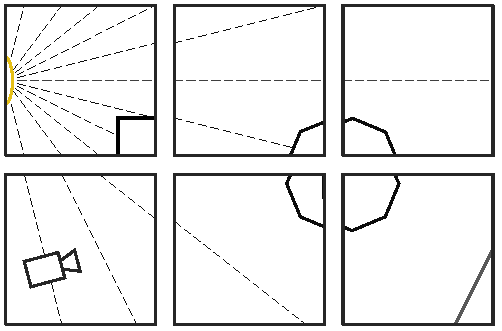
\includegraphics[width=.98\columnwidth]{drawings/Lights1.pdf}
  \caption{Initial light rays}
\end{subfigure}
\begin{subfigure}{.49\columnwidth}
 \centering
  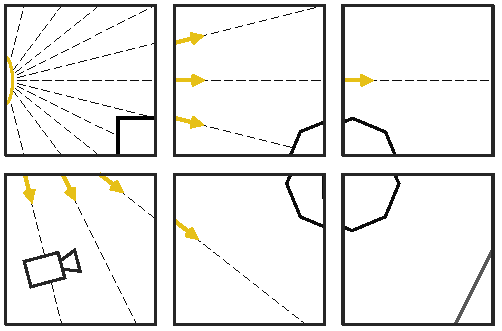
\includegraphics[width=.98\columnwidth]{drawings/Lights2.pdf}
  \caption{Point light sources}
\end{subfigure}
\caption{Light Ray Distribution}
\label{fig:light}
\end{figure}

\subsubsection{Distribute Rays}

DISTRIBUTE\_RAYS is responsible for sending each voxel its first iteration of ray information.  This is an empty set of data for all voxels except the voxel containing the camera if the camera is positioned within the domain.  If the camera is outside the domain, multiple voxels may receive data.

\subsubsection{Trace Voxel}

TRACE\_VOXEL is the heart of the application.  This step is iterative and prescribes the next iteration as long as there are rays still to trace and it has not reached a maximum threshold.  Trace voxel consumes ray packets from each of its neighbors.  It then traces the rays over its subset of the domain.  If a ray intersects with an object, secondary rays from each light source are considered if the corresponding point light source from the voxels light mesh is not in shadow.  Rays that reach the voxel walls are collected and passed to the corresponding neighbor on the next iteration.  As each CnC step instance will eventually be executed on a single node of a cluster the step code is integrating with Embree, Intel’s ray tracing kernel, in order to optimize per node performance.

\begin{figure}[!htb]
\centering
\begin{subfigure}{.49\columnwidth}
 \centering
  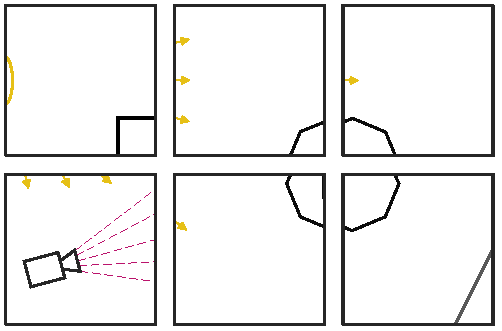
\includegraphics[width=.98\columnwidth]{drawings/Trace1.pdf}
  \caption{Distribute rays}
\end{subfigure}
\begin{subfigure}{.49\columnwidth}
 \centering
  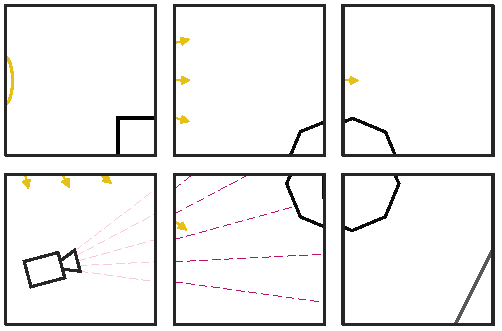
\includegraphics[width=.98\columnwidth]{drawings/Trace2.pdf}
  \caption{Trace voxel; iteration 1}
\end{subfigure}
\begin{subfigure}{.49\columnwidth}
 \centering
  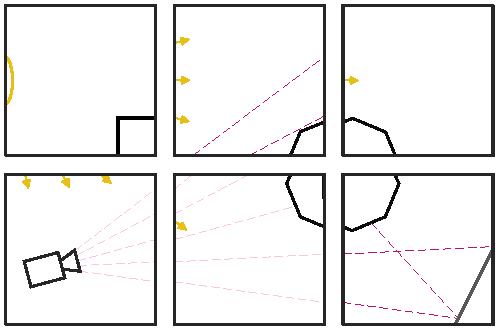
\includegraphics[width=.98\columnwidth]{drawings/Trace3.pdf}
  \caption{Trace voxel; iteration 2}
\end{subfigure}
\begin{subfigure}{.49\columnwidth}
 \centering
  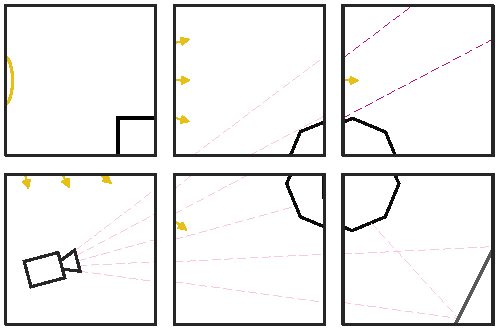
\includegraphics[width=.98\columnwidth]{drawings/Trace4.pdf}
  \caption{Trace voxel; iteration 3}
\end{subfigure}
\caption{Iterative Trace Voxel}
\label{fig:trace}
\end{figure}

\subsubsection{Produce Image}
When trace voxel has converged, a final set of ray packets will be produced.  Each ray in that packet contains the information necessary to produce the final image; merging these is the responsibility of the PRODUCE\_IMAGE step.  

\section{Future Directions}

\subsection{Hierarchy}

\subsection{Dynamic scenes}

\subsection{checkpoint and restart} 

\subsection{Global illumination}

\section{Conclusion}

%% if specified like this the section will be ommitted in review mode
\acknowledgements{
The authors wish to thank A, B, C.  CnC team at RICE? Intel?}

\bibliographystyle{abbrv}

%%use following if all content of bibtex file should be shown
%\nocite{*}
\bibliography{bibliography}{}

\end{document}
